% Created 2020-12-01 Tue 09:52
% Intended LaTeX compiler: xelatex
\documentclass[a4paper]{article}
\usepackage{graphicx}
\usepackage{grffile}
\usepackage{longtable}
\usepackage{wrapfig}
\usepackage{rotating}
\usepackage[normalem]{ulem}
\usepackage{amsmath}
\usepackage{textcomp}
\usepackage{amssymb}
\usepackage{capt-of}
\usepackage{hyperref}
\usepackage{titling}
\usepackage{xcolor}
\usepackage{float}
\usepackage{caption}
\usepackage{fullpage}
\usepackage{letltxmacro}
\usepackage{xpatch}
\usepackage{fontspec}
\usepackage[pass]{geometry}
\usepackage[newfloat]{minted}
\usepackage[square, numbers]{natbib}
\usepackage{amsmath} \usepackage{tcolorbox}\newenvironment{block}[1][]{\begin{tcolorbox}[#1,colback=blue!5,colframe=blue!40!black]}{\end{tcolorbox}}
\usepackage{xepersian}\settextfont{XB Roya}\setlatintextfont{XB Roya}\setmonofont{Iosevka}\setLTRbibitems
\def\UrlBreaks{\do\/\do-}
\xpretocmd{\verbatim}{\begin{LTR}}{}{} \xapptocmd{\endverbatim}{\end{LTR}}{}{} \xpretocmd{\minted}{\VerbatimEnvironment\begin{LTR}}{}{} \xapptocmd{\endminted}{\end{LTR}}{}{}
\LetLtxMacro{\oldmintinline}{\mintinline}\renewcommand{\mintinline}[3][]{\lr{\oldmintinline[#1]{#2}{#3}}}
\xpretocmd{\tabular}{\begin{latin}}{}{} \xapptocmd{\endtabular}{\end{latin}}{}{}
\SetupFloatingEnvironment{listing}{name=کد}
\author{\rl{مهدی صفریان}}
\date{\today}
\title{جزوه ساختمان داده}
\hypersetup{
 pdfauthor={\rl{مهدی صفریان}},
 pdftitle={جزوه ساختمان داده},
 pdfkeywords={},
 pdfsubject={},
 pdfcreator={Emacs 27.1 (Org mode 9.4)}, 
 pdflang={English}}
\begin{document}

\maketitle
\tableofcontents

\begin{block}
از انجایی که درس ساختمان داده هیچ ویدیویی ندارد و جزوه اصلی درس صرفا شامل تمارین مدرس است، فلذا توضیحات درون این جزوه فقط برداشت شخصی بنده است.
\end{block}

\section{توابع بازگشتی}
\label{sec:org81ce03f}
تابع بازگشتی تابعی است که حداقل شامل یک دستور باشد و درون خود، خودش را صدا بزند؛ توابع بازگشتی به تعداد محدود اجرا می‌شوند و پس از رسیدن به نتیجه مطلوب متوقف می‌شوند.

\subsection{مثال فاکتوریل}
\label{sec:orged4ef4e}
فاکتوریل حاصل‌ضرب اعداد \texttt{n} تا ۱ را حساب می‌کند.
برای مثال فاکتوریل عدد ۳ برابر است با \mintinline[linenos,mathescape]{latex}{3 * 2 * 1}.

\begin{listing}[H]
\caption{\label{فاکتوریل}فاکتوریل}
\end{listing}
\begin{minted}[linenos,mathescape]{python}
function fact(n) {
    if n==1                         #Fact function rules:
        return 1                    #$fact(n)=\begin{cases}1, \hspace{3.2cm} \text{n=1}.\\ n*fact(n-1), \hspace{1cm} \text{n>1}. \end{cases}$
    else
        return n * fact(n-1)
}
\end{minted}



\subsubsection{توضیحات}
\label{sec:orgd402409}
همانطور که گفته شد تابع فاکتوریل حاصل‌ضرب اعداد n تا ۱ را به دست می‌آورد. \ref{فاکتوریل}

\begin{itemize}
\item ابتدا به تابع مقداری را به عنوان ورودی می‌دهیم.
\item سپس اگر عدد ورودی تابع برابر ۱ بود، تابع متوقف شود.
\item در غیر این صورت اگر عددی غیر از ۱ بخش دوم تابع اجرا می‌شود.

مثال: فاکتوریل عدد ۴ را محاسبه کنید.
\end{itemize}

\begin{LTR}
\(fact(4)=4*3*2*1=24\)
\begin{itemize}
\item \(fact(4)= 4*fact(3)=> 4*6=24\)
\item \(fact(3)=3*fact(2)=> 3*2=6\)
\item \(fact(2)=2*fact(2)=> 2*1=2\)
\end{itemize}
\end{LTR}


\subsection{مجموع اعداد ۱ تا n}
\label{sec:org10245cc}
این تابع به سادگی همانطور که نامش مشخص است مجموع اعداد ۱ تا n را محاسبه می‌کند.

\begin{listing}[H]
\caption{مجموع اعداد ۱ تا n}
\end{listing}
\begin{minted}[linenos,mathescape]{python}
def sum(n):
    if n == 1:                    #sum function rules:
        return 1               #$sum(n)=\begin{cases}1, \hspace{3.1cm} n=1. \\ n+sum(n-1) \hspace{1cm} n>1.\end{cases}$
    else:
        print(n)
        return n + sum(n-1)
print(sum(7))
\end{minted}

مثال: مجموع اعداد ۱ تا ۳ را بیابید.

\begin{LTR}
\(sum(3)=3+2+1=6\)
\begin{itemize}
\item \(sum(3)=3+sum(2)=> 3+3=6\)
\item \(sum(2)=2+sum(1)=> 2+1=3\)
\end{itemize}
\end{LTR}

\subsection{توان}
\label{sec:orgef1a98f}
تابع توان مقدار \(n^m\) را حساب می‌کند(ورودی‌ها صحیح و مثبت هستند)
به سادگی عمل توان رسانی را حساب می‌کند.

\begin{minted}[linenos,mathescape]{python}
function power(n, m){
    if m==1                         #power function rules:
        return n                    #$power(n, m)=\begin{cases}n, \hspace{3.7cm} m=1. \\ n*power(n, m-1) \hspace{1cm} m>1.\end{cases}$
    else
        return n * power(n,m-1)

    }
\end{minted}

مثال: تابع توان را فراخوانی کنید و با مقدار دلخواه مثال بزنید.

\begin{LTR}
\(power(3,4)=> 3*3*3*3=81\)
\begin{itemize}
\item \(power(3,4)= 3*power(3,3)=3*3*3*3\)
\item \(power(3,3)= 3*power(3,2)=3*3*3\)
\item \(power(3,2)= 3*power(3,1)=3*3\)
\end{itemize}
\end{LTR}


\subsection{خارج قسمت تقسیم}
\label{sec:org9e5526c}
تابع خارج قسمت تقسیم مقدار خارج قسمت تقسیم صحیح a بر b را محاسبه می‌کند.
تاکید می‌کنم که هدف ما تقسیم صحیح است.

\begin{minted}[linenos,mathescape]{python}
def div(a,b):
    if a<b:                 #div function rules:
        return 0            #$div(a,b)=\begin{cases}0, \hspace{3.2cm} a<b. \\ div(a-b,b)+1, \hspace{1cm} a>=b. \end{cases}$
    if a>=b:
        return div(a-b,b)+1
\end{minted}

\subsubsection{توضیحات}
\label{sec:org00ab421}
\begin{itemize}
\item در مرحله اول بررسی می‌شود آیا عدد a بزرگتر از b است یا خیر.
\begin{itemize}
\item اگر کوچک‌تر باشد مقدار صفر برمی‌گردد چرا که ما مقدار تقسیم صحیح را می‌خواهیم.
\item اگر بزرگتر یا مساوی باشد عدد a برابر می‌شود با a-b و در نهایت مقدار نهایی یه واحد به آن اضافه می‌شود.
\end{itemize}
\end{itemize}

مثال: با استفاده از تابع div مقادیر a = 11 و b = 3 را بررسی کنید.

\begin{LTR}
\(div(11,3)=> 2+1=3\)
\begin{itemize}
\item \(div(11,3)= div(8,3)+1 => 2+1=3\)
\item \(div(8,3)=  div(5,3)+1 => 1+1=2\)
\item \(div(5,3)=  div(2,3)+1 => 0+1=1\)
\end{itemize}
\end{LTR}

\subsection{تابع باقی مانده تقسیم}
\label{sec:orge7f7e6d}

\begin{minted}[linenos,mathescape]{python}
def r(a,b):
    if a<b:
        return a
    else:
        return r(a-b,b)
print(r(11,3))
\end{minted}

\subsection{هانوی}
\label{sec:org4453741}
در مسئله برج هانوی ما می‌خواهیم تعداد n مهره را از میله A به C ببریم و میله B به عنوان میله کمکی استفاده کنیم.

\begin{minted}[linenos,mathescape]{python}
def tower(n, A, B, C):
    if n==1:
        return A to C
    else:
        tower(n-1, A, B, C)
        A to C
        tower(n-1, B, A, C)
\end{minted}

\subsubsection{توضیحات}
\label{sec:orgcb5eaba}
\begin{itemize}
\item ابتدا n-1 مهره را به میله B انتقال می‌دهیم و در نهایت بزرگترین مهره در A باقی می‌ماند.
\item بعد مهره بزرگ را به میله C منتقل می‌کنیم.
\item در آخر مانند مرحله اول مهره‌ها را از B به C انقال می‌دهیم.
\end{itemize}

یادتان باشد که برای انتقال مهره‌ها باید از میله‌های کمکی استفاده کنیم.
\begin{center}
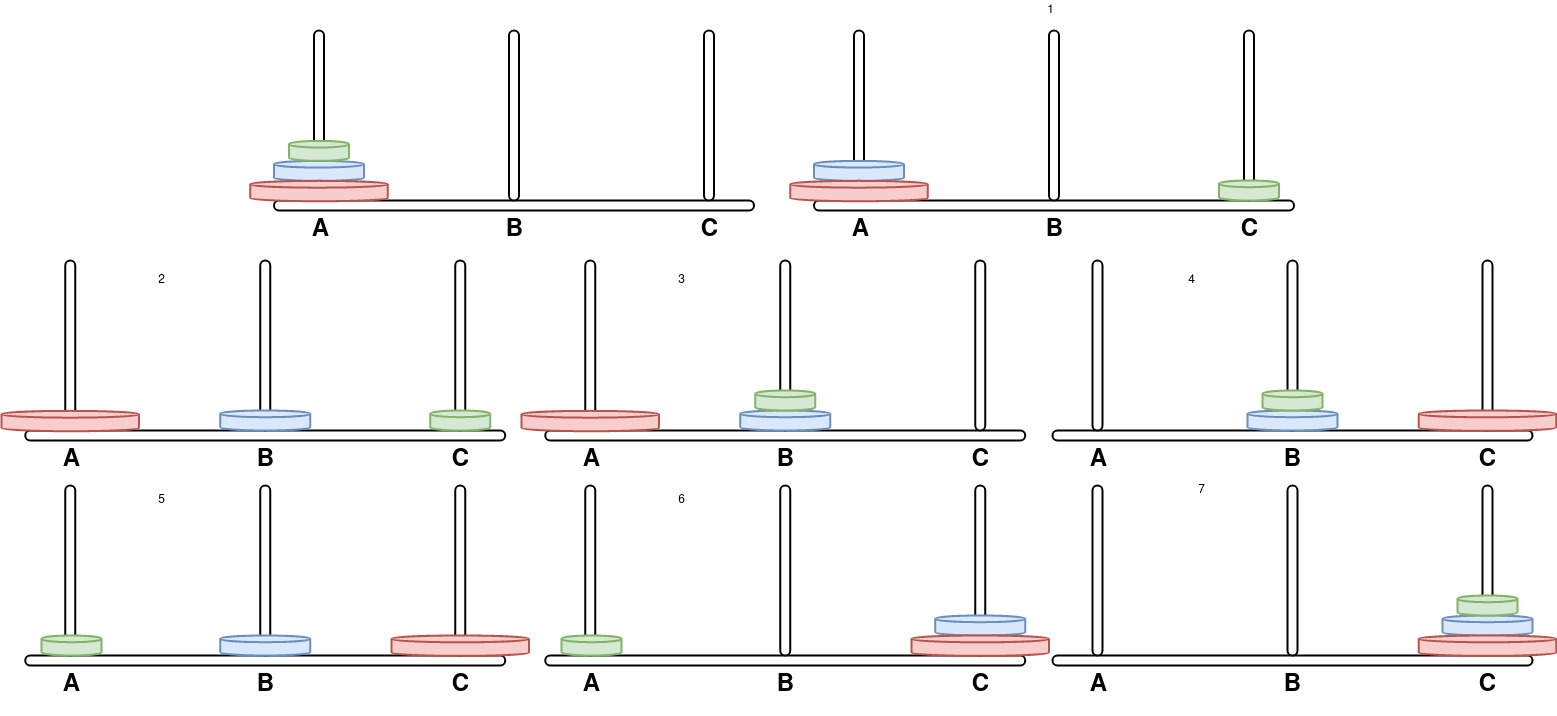
\includegraphics[width=.9\linewidth]{./tower.jpg}
\end{center}

\subsection{فیبوناچی}
\label{sec:orgfb4f6e1}
تابع فیبوناچی جمله nام اعداد فیبوناچی را به دست می‌اورد.

\begin{minted}[linenos,mathescape]{python}
def fib(n):
    if n==0 or n==1:                        #Fibonacci function rules:
        return n                            #$fib(n)=\begin{cases}n \hspace{4.4cm} 1 \\ n \hspace{4.4cm} 0 \\ fib(n-1)+fib(n-2) \hspace{1cm} n>=2 \end{cases}$
    else:
        return fib(n-1) + fib(n-2)
\end{minted}
\end{document}
